\documentclass{scrbook}
\usepackage{phd}
\newfontfamily{\pan}{code2000}
\newfontfamily{\arial}{Tahoma}

\begin{document}
\pan
 \fboxsep0pt
 \fboxrule0pt
 \parindent0pt
 \arial\par
 \raggedright
 
 \renewtcolorbox{scriptexample}[2][]{colback=black,
boxrule=0pt,toprule=0pt,colframe=white, #1}
\begin{luacode}
--- helper routines for internationalization
--  loads data from CLDR database in json format
--  and makes them available as lua.
--  Version 0.5
--  Dr Y Lazarides
--  2014.11.13


--  We use the lualibs built-in modules
--  this loads all the modules including a json converter
--

local i18n = i18n or {}
local locales = {}
local languages = {}
 
require("lualibs.lua")

-- @arg language
-- @json file
i18n.getJsonFile = function (language, file)
    local f, s
	  f = io.open('./i18n/'.. language .. '/' .. file .. '.json', 'r')
        s = f:read('*a')
        f.close()
        return s
 end

-- converts a json string to Lua
i18n.jsonToLua = function (str)
   return utilities.json.tolua(str)
end

-- loads any file into a string table
-- @arg language the language
-- @arg the file
--
i18n.load  = function (language, file)
  local str, strings
  str = i18n.getJsonFile(language, file)
  strings = i18n.jsonToLua (str)
  --tex.print(-2, strings.main[language].localeDisplayNames.scripts.Cyrl) 
  return  strings
end
 
local scripts = i18n.load('el', 'scripts') 

local calendar = require('i18n.calendar')
calendar.setLanguageDefault('Greek')

-- tex.tprint({'\\par'}, {'Default Language: ', calendar.getLanguageDefault() }, {'\\par'})

function printCalendar(month, year) 
   --  tex.tprint({calendar.months[month] },{tostring(year)} )
   calendar.makeCalendar(month, year)
end 

--printCalendar(11, 2014)

-- printCalendar(12, 2014)

function FormatDate (date)
	local dateTable = os.date ("*t", date)
	return string.format ("%02d/%02d/%04d %02d:%02d:%02d", dateTable.day, dateTable.month, dateTable.year, dateTable.hour, dateTable.min, dateTable.sec)
end

local s = FormatDate()

-- tex.print('Date: ', s)
  \end{luacode}  
 
 \def\printcalendar#1#2{%
   \luadirect{printCalendar(#1, #2)}   
 }
 
 
 
 \printcalendar{9}{2015}
 \lipsum[1]
 \vfill
  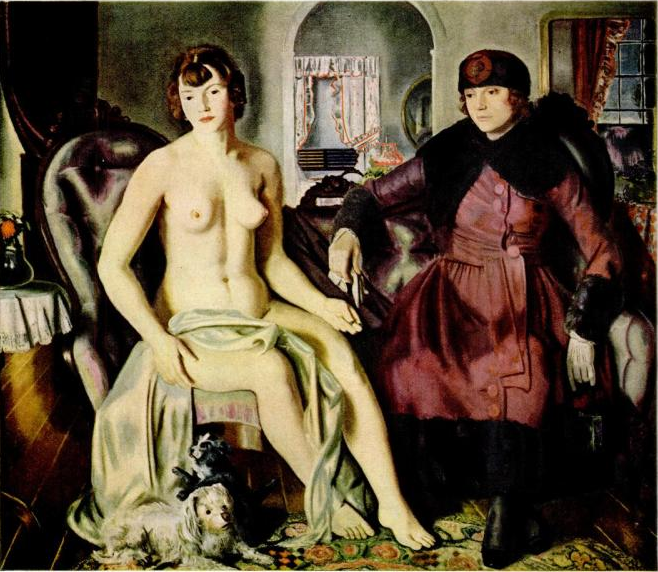
\includegraphics[width=\textwidth]{./images/twowomen-03.png}%
 \printcalendar{1}{2015}
 \lipsum[1]
 
\end{document}    
local printAll = function (language)
     local tsorted = {}
      for k,v in pairs(tmp.main[language].localeDisplayNames.territories) do
      table.insert(tsorted, k)
    end
    table.sort(tsorted)
    for k,v in ipairs(tsorted) do
      -- tex.print(v)
      tex.tprint({ v .. ' = '}, {-2, tmp.main[language].localeDisplayNames.territories[v]}, {'  \\par  '})
    end
    
   
end



i18n.printField = function (field) 
    tex.tprint({'\\par'}, {-2, field })
    tex.print('\\par')
end




-- tests

function test (locale)
   local s =  i18n.getJsonFile (locale, 'territories')
   tmp =i18n.jsonToLua(s)
   printAll(locale)
end


 
 test('cy')
 
 test('el')
 
 test('en')
 
 test('it')
 
 test('mer')
 
 test('fr-CH')
  
 test('ar')
 
 test('ne')  -- nepal
 
 test("hy") 
 
 
 test('bn') -- Bengali
 
 test('is') -- icelandic
 
 test('my')  -- Myanmar (I love Burmese scripts!)
 
 test('yo')  -- yoruba
 
 test('as') -- Assamese
 
 test('af-ZA')   -- Afrikaans south africa
 
 test('af-NA')  -- Afrikaans Nauru
 
 test('or')  -- oriya
 
  
  
 test('yi')  -- yiddish
 

 
  \end{luacode}
 
this is a test
 \end{document}
 
  locales = {'cy', 'ne', 'en'}
 for k,v in pairs (locales) do
  tex.print(i18n.printField (tmp.main['de-DE'].localeDisplayNames.territories.CY))
   tex.print(v)
 end
 
 
 
 test('ka')
\end{luacode}










\end{document}